\documentclass[final]{beamer}
\usefonttheme[onlymath]{serif}
\usepackage{subfig}
\usepackage{xcolor}
\usepackage[utf8]{inputenc}
\usetheme{SUPoster}
\usepackage{multicol}
\usepackage{diagbox}
\usepackage{tabularx}
\usepackage{booktabs}
\usepackage{todonotes}

%\usepackage[demo]{graphicx}
\usepackage{caption}
\usepackage{subcaption}


\usepackage[orientation=landscape,size=a1,scale=1.6]{beamerposter}

\captionsetup[figure]{labelformat=empty}% redefines the caption setup of the figures environment in the beamer class.
%\captionsetup[subfigure]{labelformat=empty}
\usepackage[absolute,overlay]{textpos}
\setlength{\TPHorizModule}{1cm}
\setlength{\TPVertModule}{1cm}


\usepackage{lmodern} % needed to make math mode fonts scale properly
\usepackage{url}
\usepackage{graphics}
\usepackage{bold-extra}
\usepackage{movie15}
\usepackage{caption}

\usepackage{enumitem}
% \setitemize[1]{label=$\blacktriangleright$}
% \setlist[itemize,1]{label=$\blacktriangleright$}

\setlist[itemize]{label=\usebeamerfont*{itemize item}%
  \usebeamercolor[fg]{itemize item}
  \usebeamertemplate{itemize item},
  leftmargin=1em}

% next line is necessary to make beamer and enumitem play nicely together (see http://tex.stackexchange.com/questions/45921/make-enumerate-have-beamer-themes-when-using-enumitem/45950#45950)
\setlist[enumerate]{leftmargin=2.2em,%
label=\protect\usebeamerfont{enumerate item}%
    \protect\usebeamercolor[fg]{enumerate item}%
    \insertenumlabel. }

%% DOCUMENT DATA

\title{A Formal Methods Approach Towards Deep Learning Interpretability}

\author{Kristen Kessel, Christopher Lazarus, Javier Sagastuy}
\institute{Stanford University}

\logoleft{\begin{center} 
\includegraphics[height=4.5cm]{img/SU_Seal_Blk_pos}\end{center}}
\logoright{\begin{center} 
\includegraphics[height=4.5cm]{img/icme_logo_trans} \end{center}}
\footer{CS 231N $|$ Spring 2019 \hspace{38cm} \{\texttt{kkessel, clazarus, jvrsgsty}\}\texttt{@stanford.edu}}
%
%\date{}

\begin{document}


\definecolor{almostWhite}{RGB}{240,240,240}
\definecolor{lightGray}{RGB}{220,220,220}
\definecolor{tbllinecolor}{RGB}{200,200,200}
\beamertemplateshadingbackground{lightGray}{almostWhite}
\newcommand{\vltbl}{{\color{tbllinecolor}\vrule}}


\begin{frame}[fragile]{}

%%%%%%%%%%%%%%%%%%%%%%%%%%%%%%%%%%%%%%%%%%%%%%%%%%%%%%%%%%%%%%%%%%%%
% IMPORTANT:
%   Here is where you define your poster's layout params (widths and
%   vertical positions).
%   Feel free to add/remove more, to make your layout fit your needs
%
%   All dimensions are in cm (I think).
%%%%%%%%%%%%%%%%%%%%%%%%%%%%%%%%%%%%%%%%%%%%%%%%%%%%%%%%%%%%%%%%%%%%

% centralize columns layout
\newcommand{\vstart}{58} % where the top row start vertically
\newcommand{\vstartCols}{8} % where the columns start vertically
\newcommand{\fullwidth}{81}  % this is the key to the values below
\newcommand{\colwidth}{26.5}

\newcommand{\firstcolpos}{1}
\newcommand{\secondcolpos}{28.75}
\newcommand{\thirdcolpos}{56.5}
\newcommand{\bottomblockstart}{108.5}


% this will add some padding to the blocks, to avoid text reaching
% the border (looks bad)
\newenvironment{paddedBlock}[2][0.95\linewidth]
    {\begin{block}{#2}\begin{minipage}{#1}}
    {\end{minipage}\end{block}}

%%%%%%%%%%%%%%%%%%%%%%%%%%%%%%%%%%%%%%%%%%%%%%%%%%%%%%%%%%%%%%%%%%%%
% And now ... the content
%%%%%%%%%%%%%%%%%%%%%%%%%%%%%%%%%%%%%%%%%%%%%%%%%%%%%%%%%%%%%%%%%%%%

%%%%%%%%%%%%%%%%%%%%%%%%%
%%%%%%%%%%%%%%%%%%%%%%%%%
%% LEFT COLUMN
%%%%%%%%%%%%%%%%%%%%%%%%%
%%%%%%%%%%%%%%%%%%%%%%%%%
\begin{textblock}{\colwidth}(\firstcolpos,\vstartCols)

\begin{paddedBlock}{Summary}
Although deep neural networks have proved to be very successful at classification tasks, their intrinsic complexity makes reasoning about a classification outcome difficult.
In recent work [2], statistical methods were introduced as a means to assess the influence of human-intelligible concepts in classification outcomes.
We aim to assess and extend such methods by leveraging formal methods for neural network verification.
\begin{itemize}
\item \textbf{Question:} How important is a concept in classifying image $i$ as label $k$? e.g. Is the presence of stripes relevant in the classification of an animal as a zebra?
\item \textbf{Approach \#1:} Use TCAV framework to provide statistical guarantees
\item \textbf{Approach \#2:} Use neural network verification methods [1] to provide formal guarantees
\end{itemize}
\end{paddedBlock}

\begin{paddedBlock}{Testing with Concept Activation Vectors (TCAV) [2]}
\begin{itemize}
\item \textbf{Idea:} Identify the region in the latent space corresponding to layer $\ell$ of the network in which a human-intelligible concept (e.g. blue) manifests more intensely with a vector called the Concept Activation Vector (CAV). Measure the relevance of this concept for classification of image $i$ as class $k$ by taking directional derivative of the layer $\ell$ activations for image $i$ with the CAV.
\item \textbf{Inputs:}
	\begin{itemize}
	\footnotesize{
	\item trained classification network
	\item set of examples for a user-defined concept $C$ and set of random counterexamples
    \item labeled examples for the class $k$ under consideration
    }
	\end{itemize}
\item \textbf{Outputs:}
	\begin{itemize}
	\footnotesize{
	\item CAV $v_c^\ell$ for concept $C$ at layer $\ell$
    \item TCAV score $S_{C,k}^\ell(\mathbf{x})$ of the sensitivity of the model's prediction of class $k$ to concept $C$
    	\[ S_{C,k}^\ell(\mathbf{x}) = \nabla h_k^\ell\left(f_\ell(\mathbf{x})\right) \cdot \mathbf{v}_C^\ell \]
    \item $p$-value testing the hypothesis that concept $C$ is not relevant in classifying images of class $k$
    }
	\end{itemize}
\end{itemize}
%\vspace{-5mm}
\end{paddedBlock}

\begin{paddedBlock}{Neural Network Verification}
\[ \vec x\in \mathcal{X} \Rightarrow \vec y=\vec f(\vec x)\in \mathcal{Y} \]
\end{paddedBlock}
\end{textblock}

%%%%%%%%%%%%%%%%%%%%%%%%%
%%%%%%%%%%%%%%%%%%%%%%%%%
%% RIGHT COLUMN
%%%%%%%%%%%%%%%%%%%%%%%%%
%%%%%%%%%%%%%%%%%%%%%%%%%
\begin{textblock}{\colwidth}(\secondcolpos,\vstartCols)
\begin{paddedBlock}{Approach: TCAV + Verification}
%\vspace{8mm}

\alert{Custom Data Sets}
%\begin{figure}%
%    \centering
%    \subfloat[label 1]{{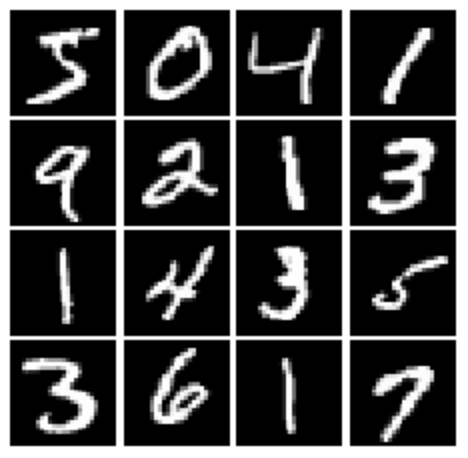
\includegraphics[width=5cm]{img/mnist_bw.png} }}%
%    \qquad
%    \subfloat[label 2]{{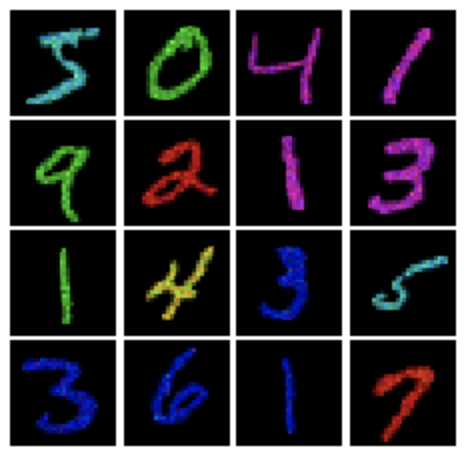
\includegraphics[width=5cm]{img/mnist_color.png} }}%
%    \caption{2 Figures side by side}%
%    \label{fig:example}%
%\end{figure}

\begin{figure}%
    \centering
    \subfloat[Colorized MNIST training set for classification of hand-written digits]{{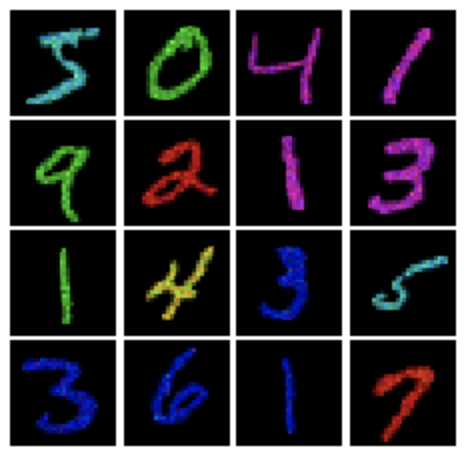
\includegraphics[width=5cm]{img/mnist_color.png}}}%
    \qquad
    \subfloat[Blue concept training set and non-blue training set to learn CAVs for concept blue]{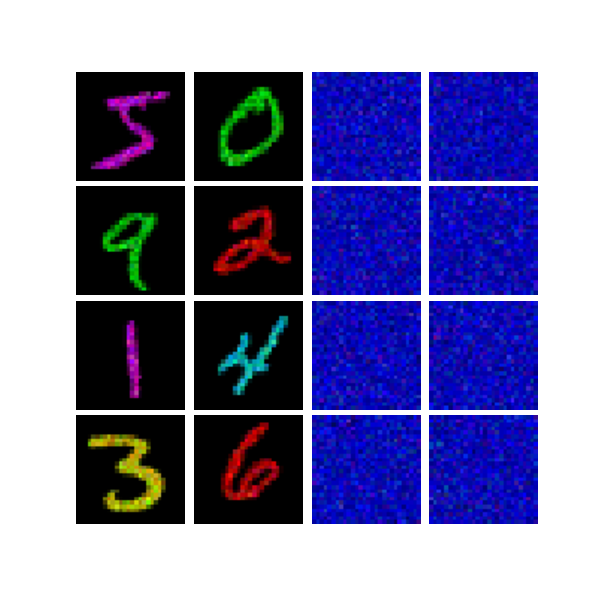
\includegraphics[width=.2\textwidth]{img/cav_viz}}}%
    \qquad
    \subfloat[blah blah]{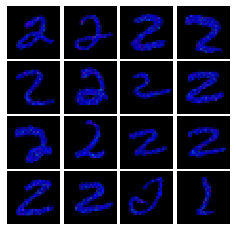
\includegraphics[width=.2\textwidth]{img/blue2s}}
%    \caption{2 Figures side by side}%
    \label{fig:example}%
\end{figure}

%\begin{figure}
%    \centering
%    %\missingfigure[width=0.5\textwidth]{2 graphs fig}
%    %\missingfigure{Hallucigraph architecture sketch}
%    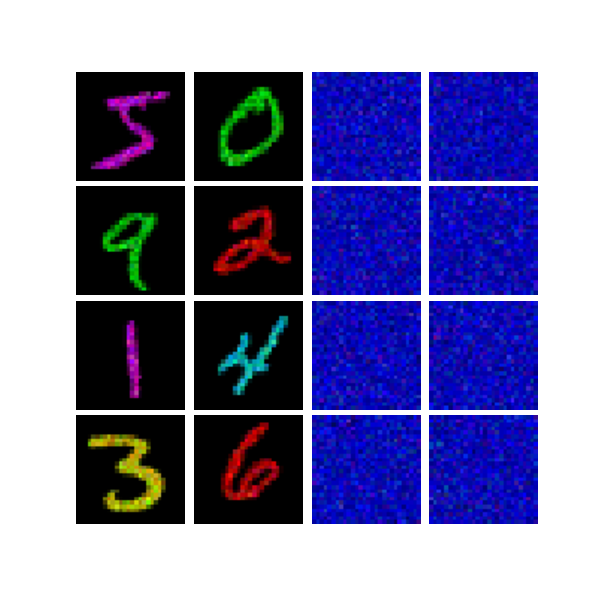
\includegraphics[width=.2\textwidth]{img/cav_viz}
%    %\caption{Caption}
%    \label{fig:big}
%\end{figure}

%\vspace{8mm}

\alert{Maybe talk about classe sand support vector}
LALALALALAL

\begin{figure}%
    \centering
    \subfloat[label 1]{{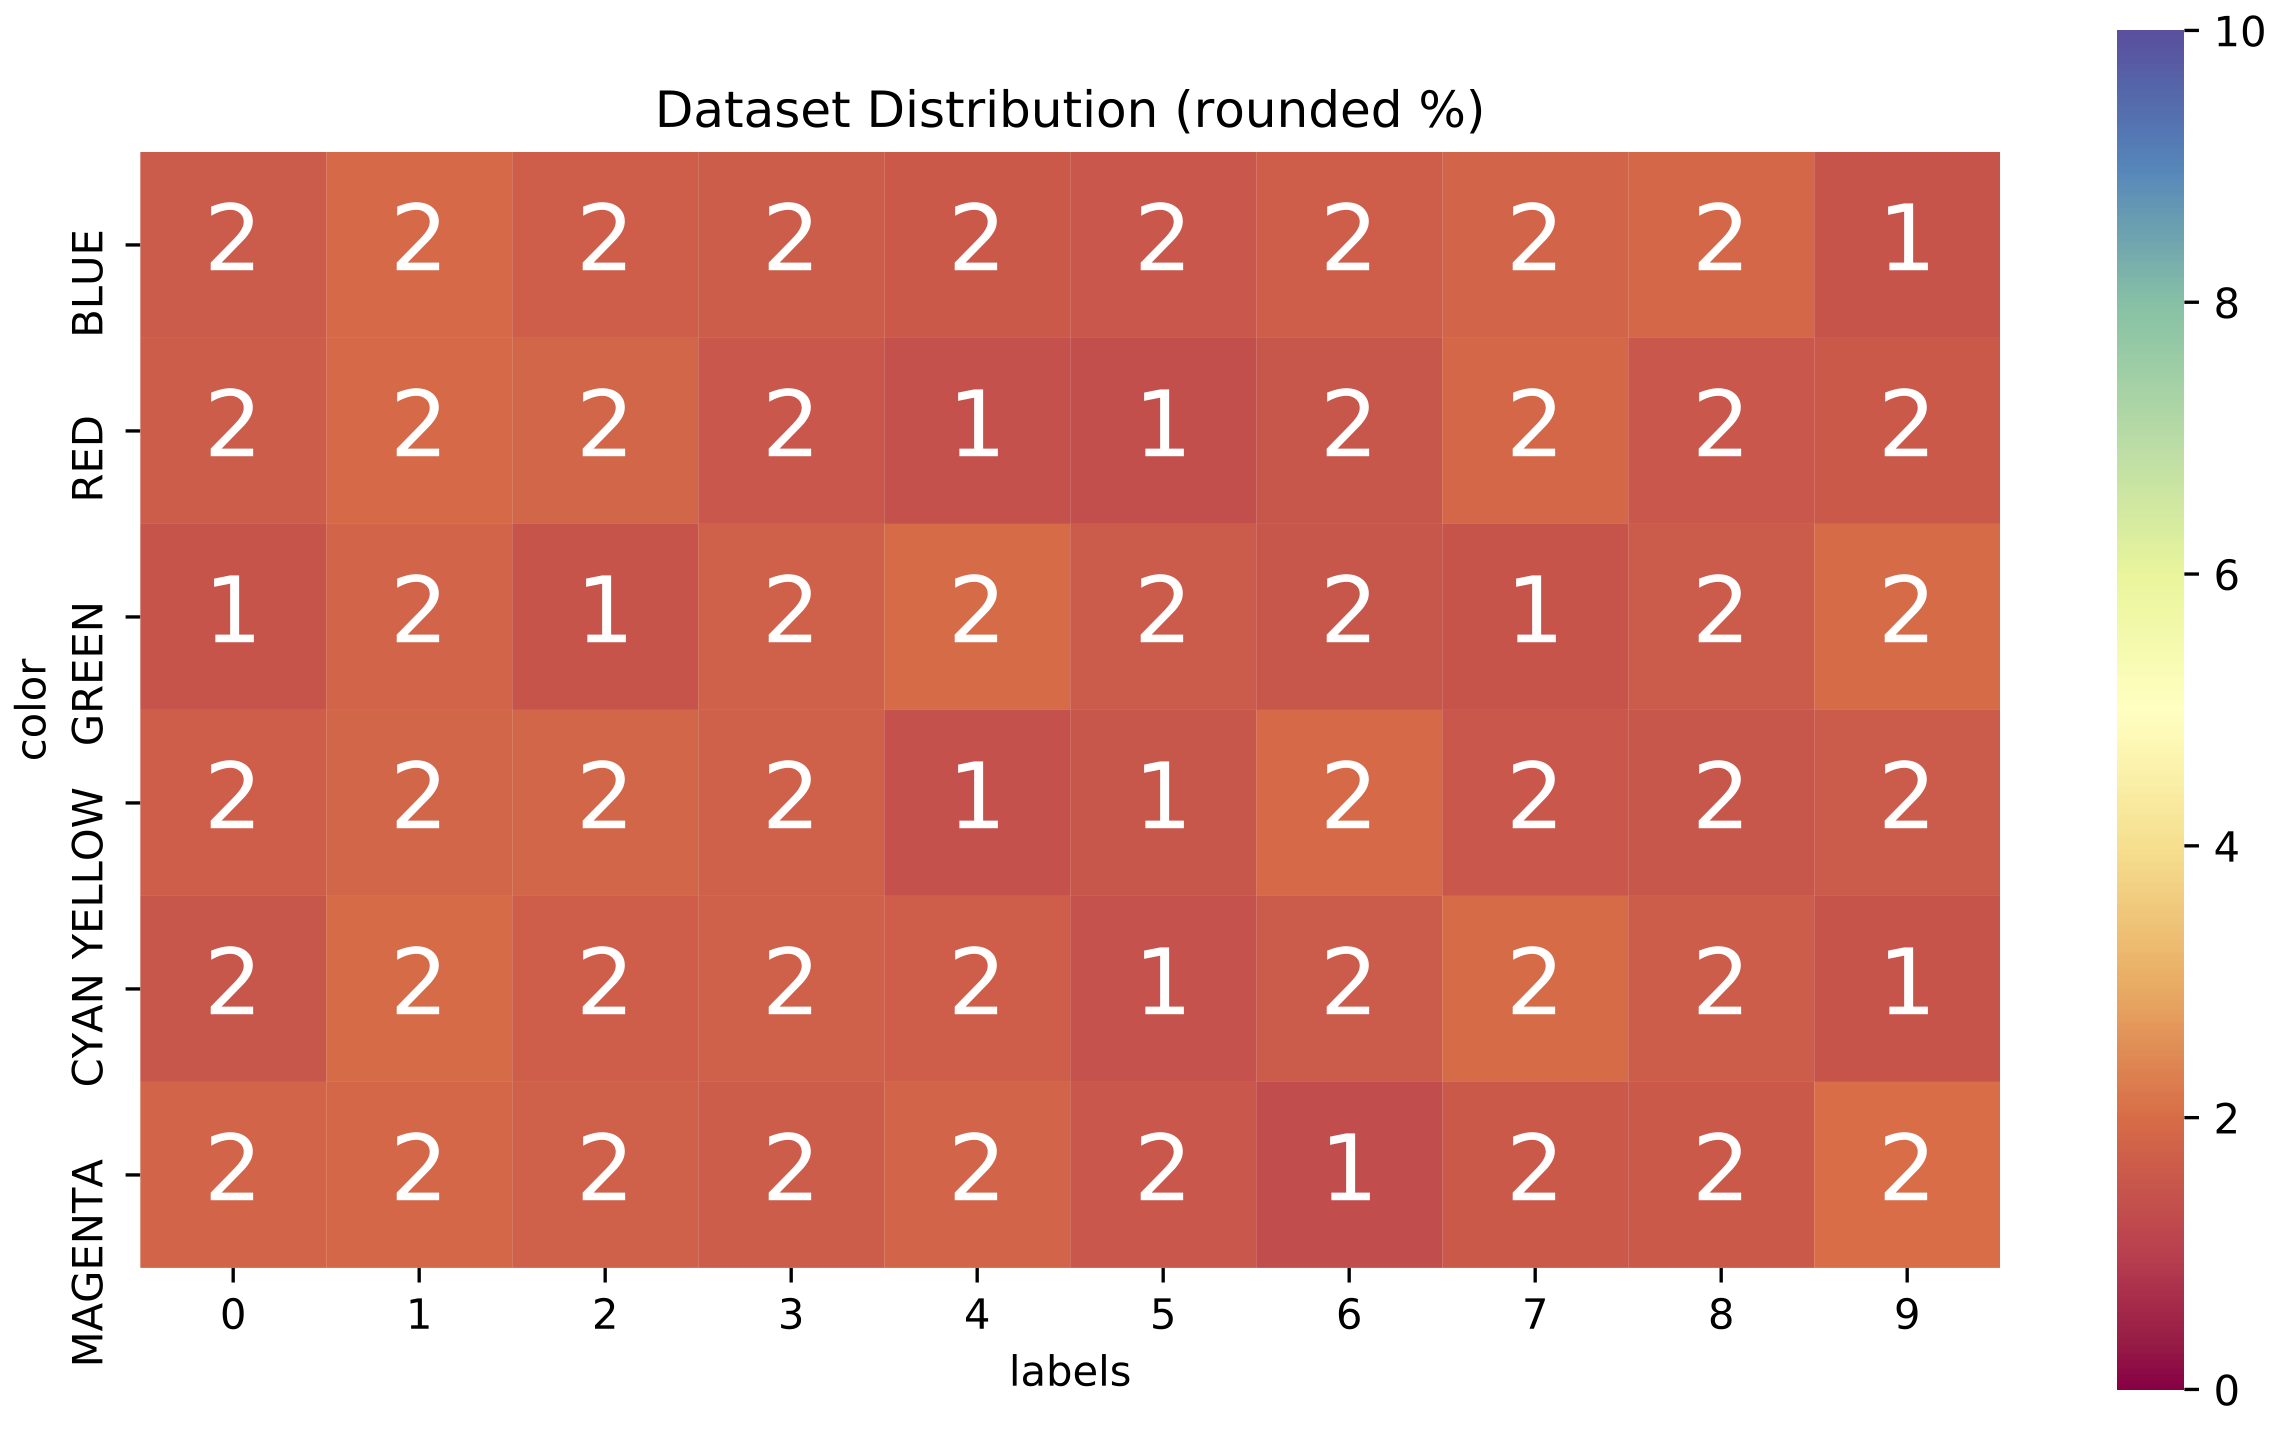
\includegraphics[width=.4\textwidth, backgroundcolor=white]{img/data_distr_balanced_test_new2} }}%
    \qquad
    \subfloat[label 2]{{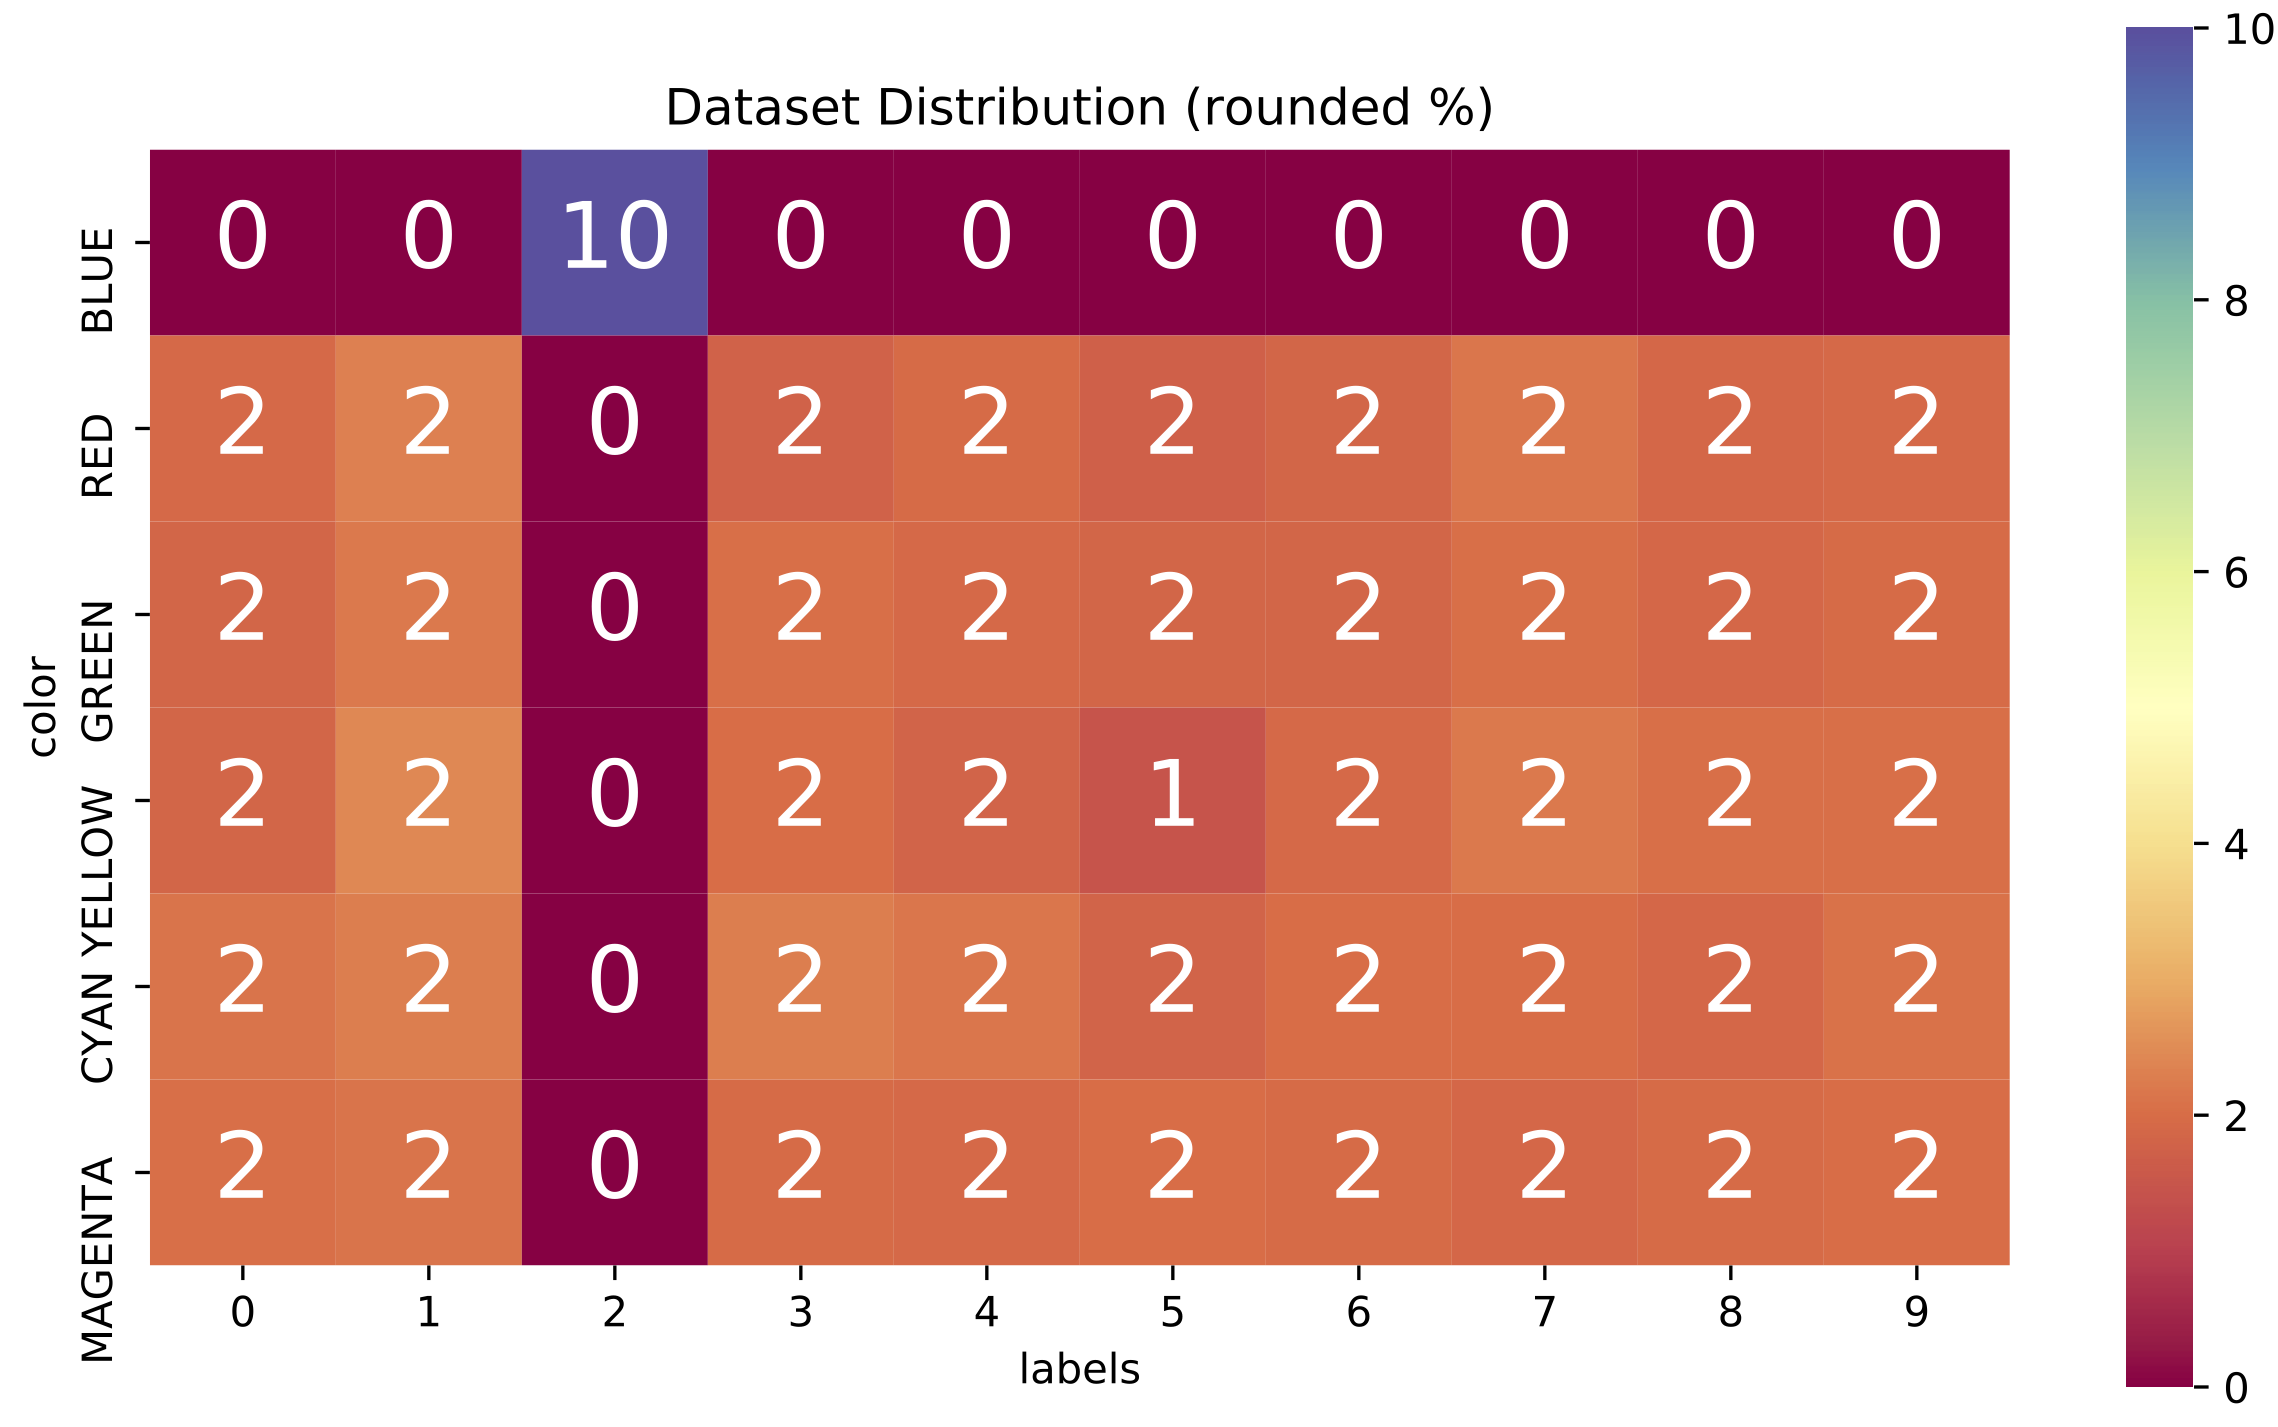
\includegraphics[width=.4\textwidth]{img/data_distr_blue2_test_new2} }}%
    \caption{2 Figures side by side}%
    \label{fig:example}%
\end{figure}


\begin{align*}
\mathcal{L}_{LP}=&-\mathbb{E}_{Z\sim q(Z|A,X)}[A_{ij}\mathrm{log}\tilde{A}_{ij}+(1-A_{ij})\mathrm{log}(1-\tilde{A}_{i,j})]\\
&+\mathrm{KL}(q(Z|A,X)||p(Z)).
\end{align*}
%\vspace{-8mm}

%\vspace{8mm}
\alert{2. Edge hallucination}
  produces $\hat{A}$:
  \begin{itemize}
    \item top$K$ ($K$ hyper-parameter)
    \item sampling using gumbel softmax [4] trick (allows gradients to flow)
  \end{itemize}
\alert{3. Node classification}
\begin{itemize}
	\item $\hat{y} = \mathrm{GCN}(\hat{A}, X)$
\end{itemize}

\end{paddedBlock}
%\vspace{3mm}
\end{textblock}


\begin{textblock}{\colwidth}(\thirdcolpos,\vstartCols)

%\begin{paddedBlock}

%\
%$\hat{y}=\mathrm{GCN}(\hat{A}, X)$

%\end{paddedBlock}

\begin{paddedBlock}{Results}
%\vspace{8mm}

\alert{Need to talk about significant CAVs}
Then talk about the avenues and boulevards.

\begin{figure}
    \centering
    %\missingfigure[width=0.5\textwidth]{2 graphs fig}
    %\missingfigure{Hallucigraph architecture sketch}
    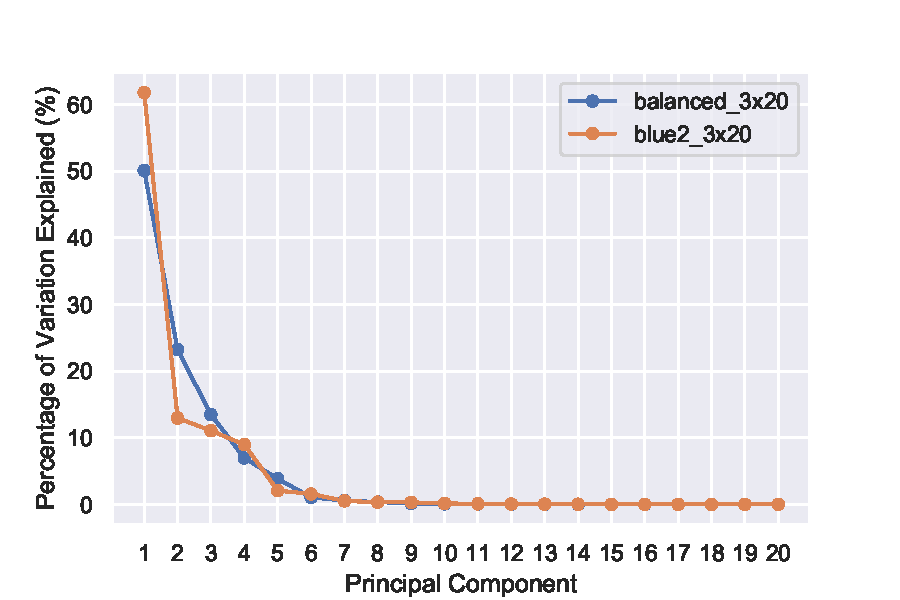
\includegraphics[width=.8\textwidth]{img/scree_plot}
    %\caption{Caption}
    \label{fig:big}
\end{figure}

%\vspace{8mm}
\alert{Node classification results}

\begin{table}
\centering
\begin{tabular}{lcccc}
\hline

\textbf{model} &  \textbf{balanced} &   \textbf{blue 2} &    \textbf{red 2} &  \textbf{green 2} \\ \hline 
\texttt{balanced\_5x50} &    $0.942$ &  $0.942$ &  $0.941$ &  $0.944$ \\
\texttt{blue2\_5x50} &    $0.780$ &  $0.952$ &  $0.682$ &  $0.689$ \\
\texttt{balanced\_3x50} &    $0.942$ &  $0.940$ &  $0.942$ &  $0.941$ \\
\texttt{blue2\_3x50} &    $0.724$ &  $0.954$ &  $0.675$ &  $0.684$ \\
\texttt{balanced\_3x20} &    $0.890$ &  $0.890$ &  $0.891$ &  $0.888$ \\
\texttt{blue2\_3x20} &    $0.708$ &  $0.923$ &  $0.663$ &  $0.672$ \\
\hline

\end{tabular}
\end{table}



\begin{itemize}
  \item Try to salvage somethibg
  \item Nothing worked : )
\end{itemize}

\end{paddedBlock}


\begin{paddedBlock}{References}
\footnotesize{[1] G. Katz, C. Barrett, D. L. Dill, K. Julian, and M. J. Kochenderfer. Reluplex: An efficient smt solver for verifying deep neural networks. In International Conference on Computer Aided Verification, pages 97–117. Springer, 2017}

\footnotesize{[2] B. Kim, M. Wattenberg, J. Gilmer, C. J. Cai, J. Wexler, F. B. Viegas, and R. Sayres. Interpretability beyond feature attribution: Quantitative testing with concept activation vectors (tcav). In ICML, 2018}

\footnotesize{[3] Y. LeCun, C. Cortes, and C. Burges. Mnist handwritten digit database. AT&T Labs [Online]. Available: http://yann. lecun. com/exdb/mnist, 2:18, 2010}

\footnotesize{[4] C. Liu, T. Arnon, C. Lazarus, C. Barrett, and M. J. Kochenderfer. Algorithms for verifying deep neural networks. CoRR, abs/1903.06758, 2019}

\end{paddedBlock}
\end{textblock}


%%%%%%%%%%%%%%%%%%%%%%%%%
%%%%%%%%%%%%%%%%%%%%%%%%%
%% BOTTOM ROW
%%%%%%%%%%%%%%%%%%%%%%%%%
%%%%%%%%%%%%%%%%%%%%%%%%%

%\begin{textblock}{\fullwidth}(2,\bottomblockstart)
%\begin{paddedBlock}[0.98\linewidth]{Acknowledgements}

%In case you need it, you can do this too

%\end{paddedBlock}
%\end{textblock}

\end{frame}
\end{document}
